%% PNAStwoS.tex
%% Sample file to use for PNAS articles prepared in LaTeX
%% For two column PNAS articles
%% Version1: Apr 15, 2008
%% Version2: Oct 04, 2013

%% BASIC CLASS FILE
\documentclass{pnastwo}

%% ADDITIONAL OPTIONAL STYLE FILES Font specification

%\usepackage{pnastwoF}



%% OPTIONAL MACRO DEFINITIONS
%\def\s{\sigma}
%%%%%%%%%%%%
%% For PNAS Only:
%\url{www.pnas.org/cgi/doi/10.1073/pnas.0709640104}
%\copyrightyear{2008}
%\issuedate{Issue Date}
%\volume{Volume}
%\issuenumber{Issue Number}
%\setcounter{page}{2687} %Set page number here if desired
%%%%%%%%%%%%

\begin{document}

\title{Agreement on Characterization between Transformative Works}

\author{Yizhi Jing\affil{1}{Indiana University Bloomington},
}

\contributor{2015Fall I590 Final Paper}

\maketitle

\begin{article}
\begin{abstract}
{In this paper I present a study about the development of agreement on characterization of fictional characters witnin fandom communities with analysis of transformative works that they produce. Based on data of a major fandom community that developed within the past a few years,  text analysis with deep learning methods show that while writings about a character remains fairly similar, especially in short terms, in long terms a higher level of diversity may be identified. Meanwhile,  abstraction to the sentiment level indicates that although considerable divergence remains between creators, the agreement level tend to increase over time. Analysis with tags that summarizes these works suggest that while the frequency of most frequent tags correlates mainly with the amount of works, tags with the highest and lowest popularity have peaks in certain time periods that does not correspond to the overall distribution, implying the possibility of diffusion processes within the community. }
\end{abstract}

\keywords{text analysis | social systems | }

Among the many types of dynamics in online communities, consensus of opinion is one that captures multiple kinds of interaction, and exhibits different forms . In some communities, formal mechanisms for resolving discrepancies are provided: for example, Wikipedia provides discussion pages for every entry [cite wiki], where editors attempt to reach agreement on how the entry should be written. However, in many other situations, this process takes place in more subtle ways, and are more difficult to trace. [cite something]

In this work, I focus on a specific kind of online communities - fandoms. Fandom communities, by convention, are a group of people that identify, connect and interact with each other based on a similar interest, such as a movie, a book or a band [cite https://en.wikipedia.org/wiki/Fandom]. While many of the major events, such as comic-cons, happen offline, many fans devote a large portion of fandom activities online.

Transformative works, or fan works, are one typical kind of production from fandom communities. These are creative works made by fans based on one or more original works, and are often centered around certain characters or story lines. For example, a fiction written by a contemporary fan about Sherlock Holmes in his retirement is considered a fan fiction in the Sherlock Holmes fandom. By this nature, these works reflect the understanding of the creators about the characters and the story, which differs from person to person and changes over time.

I base my work on the assumption that analysis of transformative works may reveal the development of consensus of opinion between fans. In particular, this development may correspond to the typical life stages of a fandom, such as its origin, growth, decline and death. Intuitively, we may find two ways to describe this process that are both reasonable: it is possible that when the fandom grows and matures, common knowledge emerges between its members and the agreement level becomes higher. However, it is also possible that as the size of the fandom increases, or because of other external events, more diversity will be introduced. It is this work's objective to quantitatively frame, and analyze these assumptions.

The data for this analysis comes from the online transformative work archive site Archive of Our Own (AO3)[cite: http://archiveofourown.org/]. This site allows users to freely upload their works, and categorizes them based on fandoms. It also utilizes a metadata system to store these works' information, allowing for many filtering and classifying operations. Established in 2010, it has become one of the most popular transformative work archives.

As a starting point, the project is limited to only 1 fandom: \textit{Sherlock(TV) }, the BBC TV series starring Benedict Cumberbatch and Martin Freeman. It is chosen as the case for study because of two reasons: first, it is among the fandoms with largest amounts of data, covering $~3\%$ of all works on the site with 77, 510 works. Secondly, AO3 opened on January 1st 2010, while the first episode of \textit{Sherlock} was broadcasted  on July 2010, which implies that the archive was able to record the origin and growth of the fandom. 



\section{Method}
The data collected from the website includes 75,694 transformative works from the fandom described above, 
with publish date ranging from July 2010 to November 2015. Number of words in this dataset is 405,230,386. 
Besides the work texts, the metadata collected include 20 fields that can be roughly divided into two categories: some are generated by the author, which describes the work's content; others are automatically generated, and describes other work information, as well as the readers' feedback. Table 1 gives the names of these fields. The time distribution of works published is shown in Figure \ref{time_work}, along with major events in the fandom, such as the broadcasting of a new season of the series. 

\begin{figure}
\centerline{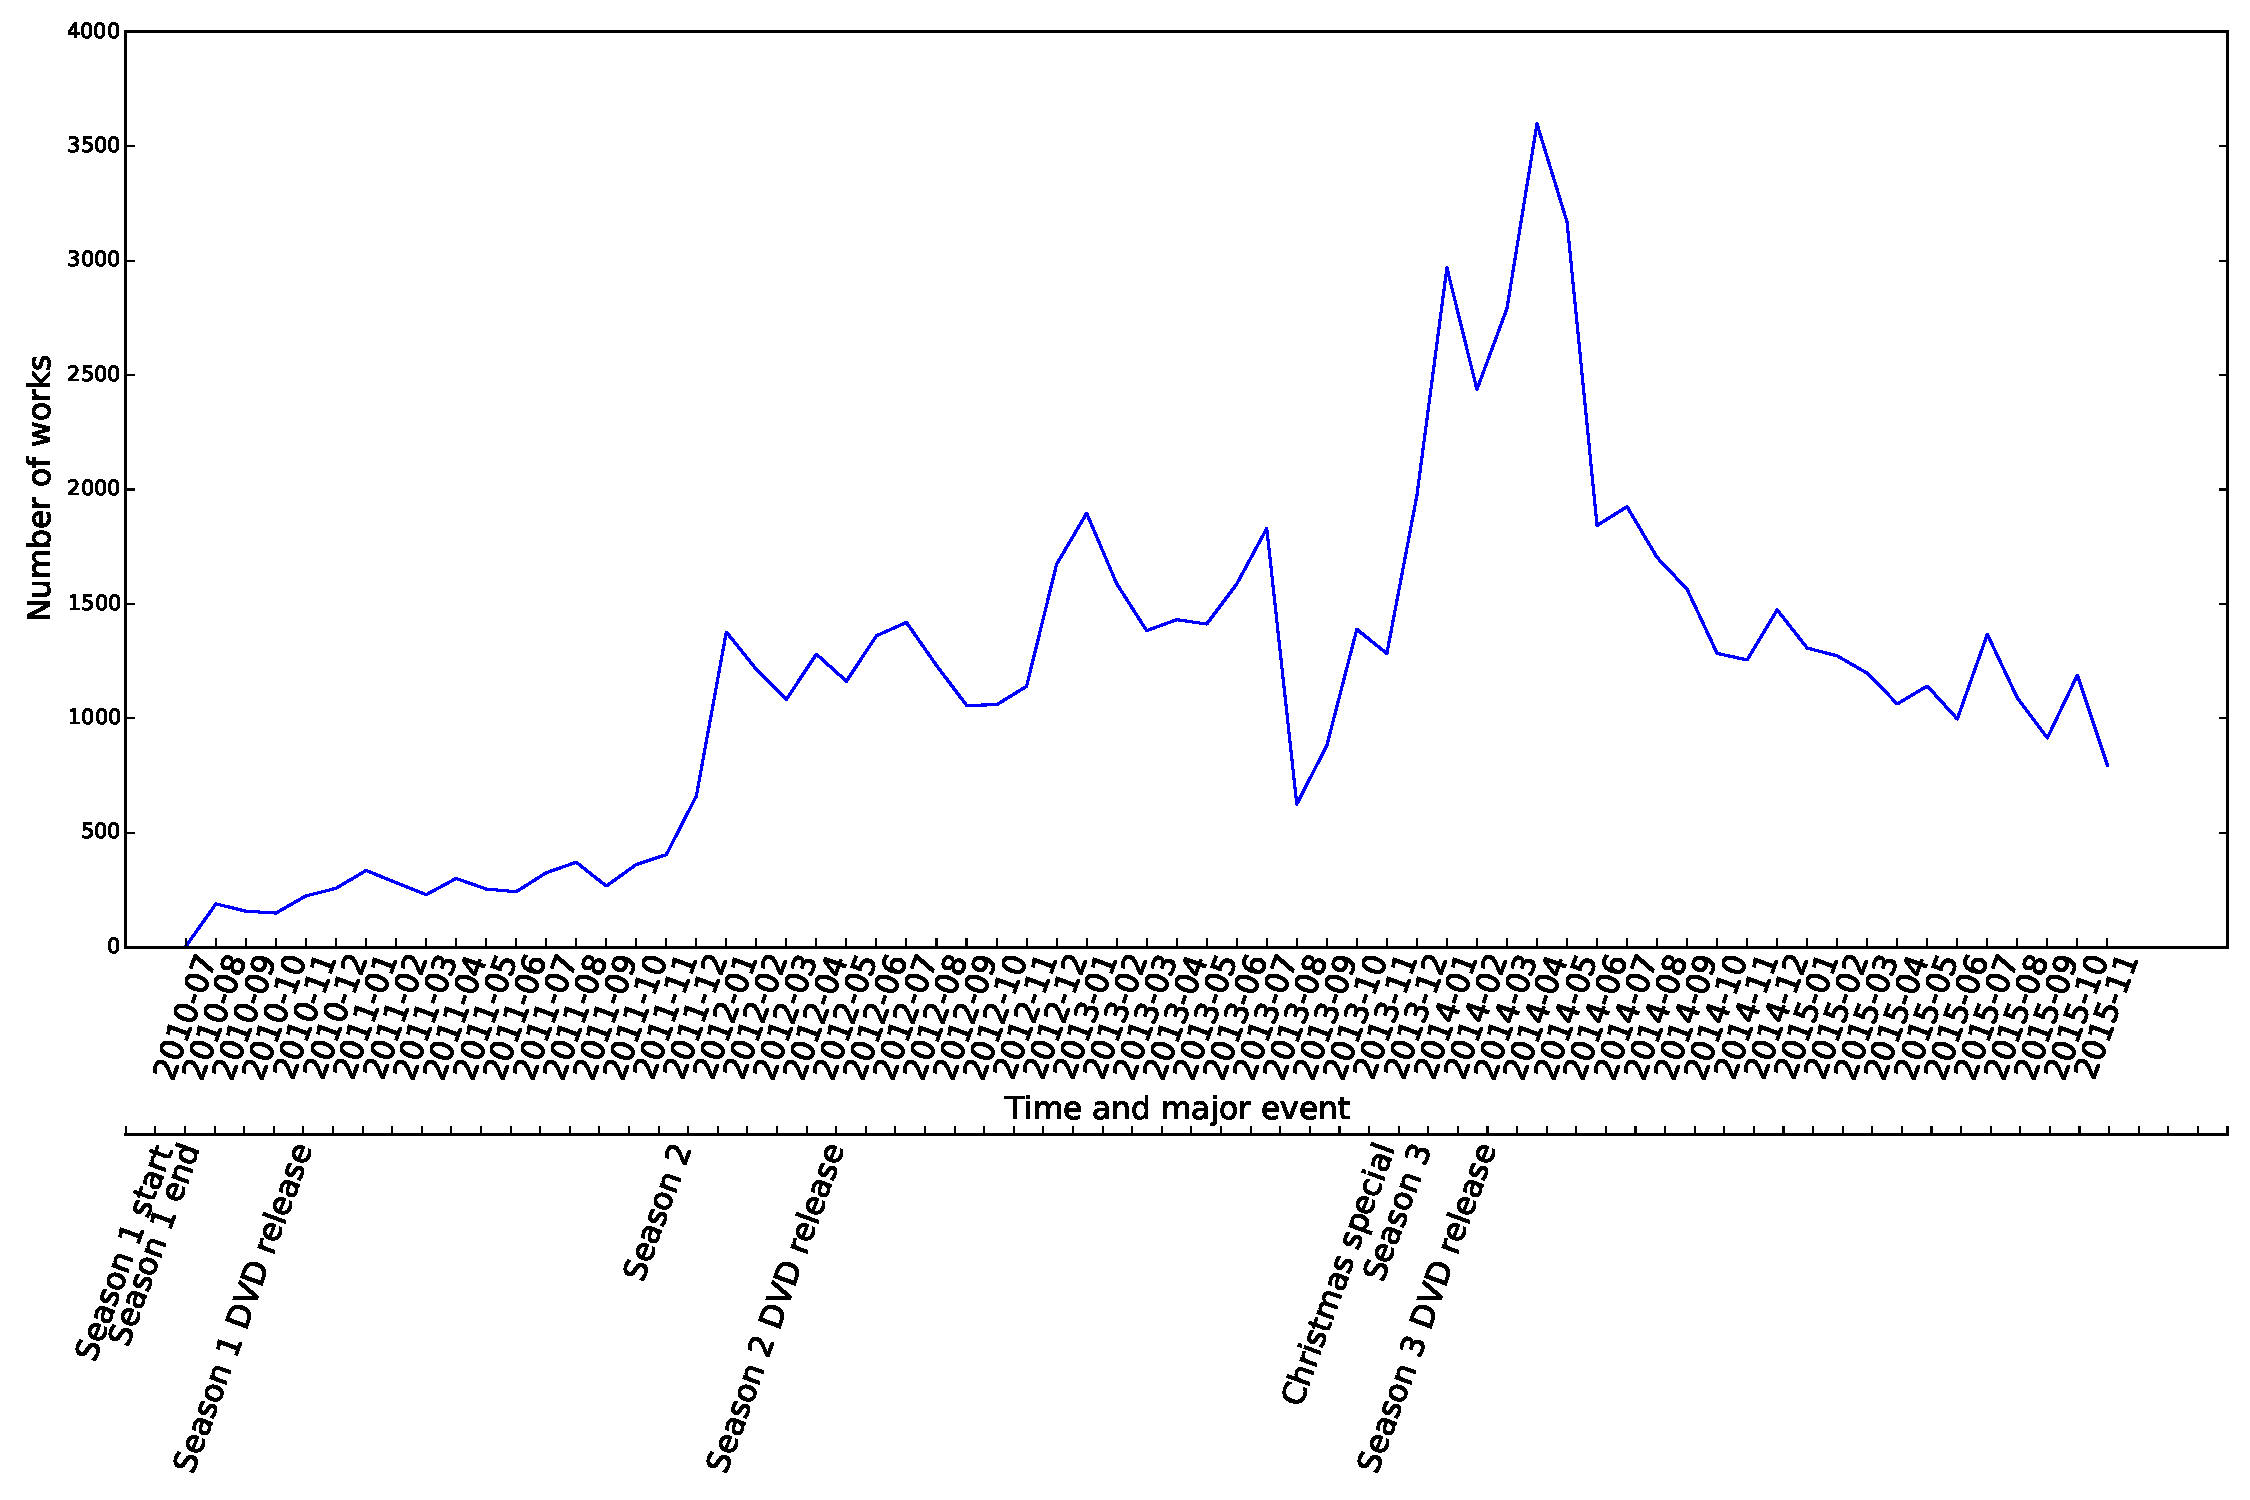
\includegraphics[width=.5\textwidth]{time_work.pdf}}
\caption{Time distribution of works published.}\label{time_work}
\end{figure}

The original plan includes extracting parts of the work texts that provides more information on characterization. 
There have been works that approach this objective from researchers in computational linguistics, narratology and morphology[cite the 3-4 papers]. however, it seems that current state-of-arts models are yet to provide simple and robust methods, and it may be risky to base further analysis on these results if complicated methods are introduced. Therefore, I chose to apply simpler methods, in order to achieve a higher level of abstraction of the works.

I first applied the word2vec algorithm to extract words that are most closely related to a given character. Introduced by <>, this model has gained a lot of popularity in the past a few years[cite original paper]. It trains a neural network with the text, and is available to capture the words' context. As a result, it is able to identify words that occur with a similar pattern.

The works are first grouped by their publish time (year/month), constructing time slices of the dataset, which includes 65 months. The count of words per slice is therefor around 6 million, which may be a bit small for training the word2vec model. However, examination of the results suggest that it is able to capture similarities in a reasonable way. I then search for words that are mostly related to a given character (such as "Sherlock" or "Moriaty", and record the top words. 

These word sets are then used to construct a document-word matrix, in which the top words of each month are considered as documents. To compare the change of similarity between works of different time periods, I chose to use the mutual information between two documents. This metric captures, in a sense, to what degree we can use one document to predict the other. It is calculated as following:

[MI formula]

Another possible approach to extract information from the texts to a more abstract level is through sentiment analysis. For this I applied the lexicon-based approach, which gives each word in the lexicon a score that describes its positiveness or negativeness. The lexicon used is from Mitchell et al's work that analyses Twitter's 
sentiment, the words from which was rated by Amazon Mechanical Turks. 

I then calculate the works' average sentiment scores by taking average over the words in the text that can be found in the lexicon, and categorize them into 3 categories (positive, negative and neutral). Following similar works from [cite the sentiment arc papger], only sentences in which only a given character appears are considered.  For each time period, I record the number of works in the subset that are labeled as positive and negative, respectively. To estimate the agreement between authors, I calculate the Fleiss' kappa of these time periods. In the calculation, each author is considered as a rater[cite wiki page], and the kappa value captures the degree of agreement on the categories that their works fall into. The kappa is defined as:

[formula]

Besides analysis on the text level, another approach is to work with the works' tags. These are created by the authors, and describes certain settings, memes and plots in a given work. In a sense, they are like tropes that captures specific narrative elements in the works.  It seems possible that the popularity of a tag can be an indicator of how much people are acceptive of it, and therefore, people's agreement on this trope. The popular tags are identified in two ways: one is simply the frequency of its occurrence, and the second is to measure by the average kudos (likes) that a work with this tag received. In the second case, tags are filtered by occurrence with a threshold of 100, as a way to reduce bias. 




\section{Results}
\subsection{Mutual Information} Figure \ref{mi_pearson} shows the mutual information between every two successive months of words related to John Watson. The mutual information is adjusted against chance. Pearson correlation between each pair of word distributions are also plotted for comparison. It can be seen that while these two metrics correlates fairly well with each other,  different patterns can also be noticed.

To better understand the pattern of mutual information changes, I also calculate the mutual information with multiple step lengths. The steps are defined as months, so that 2-step mutual information means the mutual information between this month and two months later, etc. Figure \ref{multi_mi} shows the 1-4 steps mutual information changes. It seems that the 2-step and 3-step comparisons are able to reveal a more clear pattern, showing a gradual increase and then fluctuating decrease, which may suggest that more diversity was introduced into the scene. 


\begin{figure}
\centerline{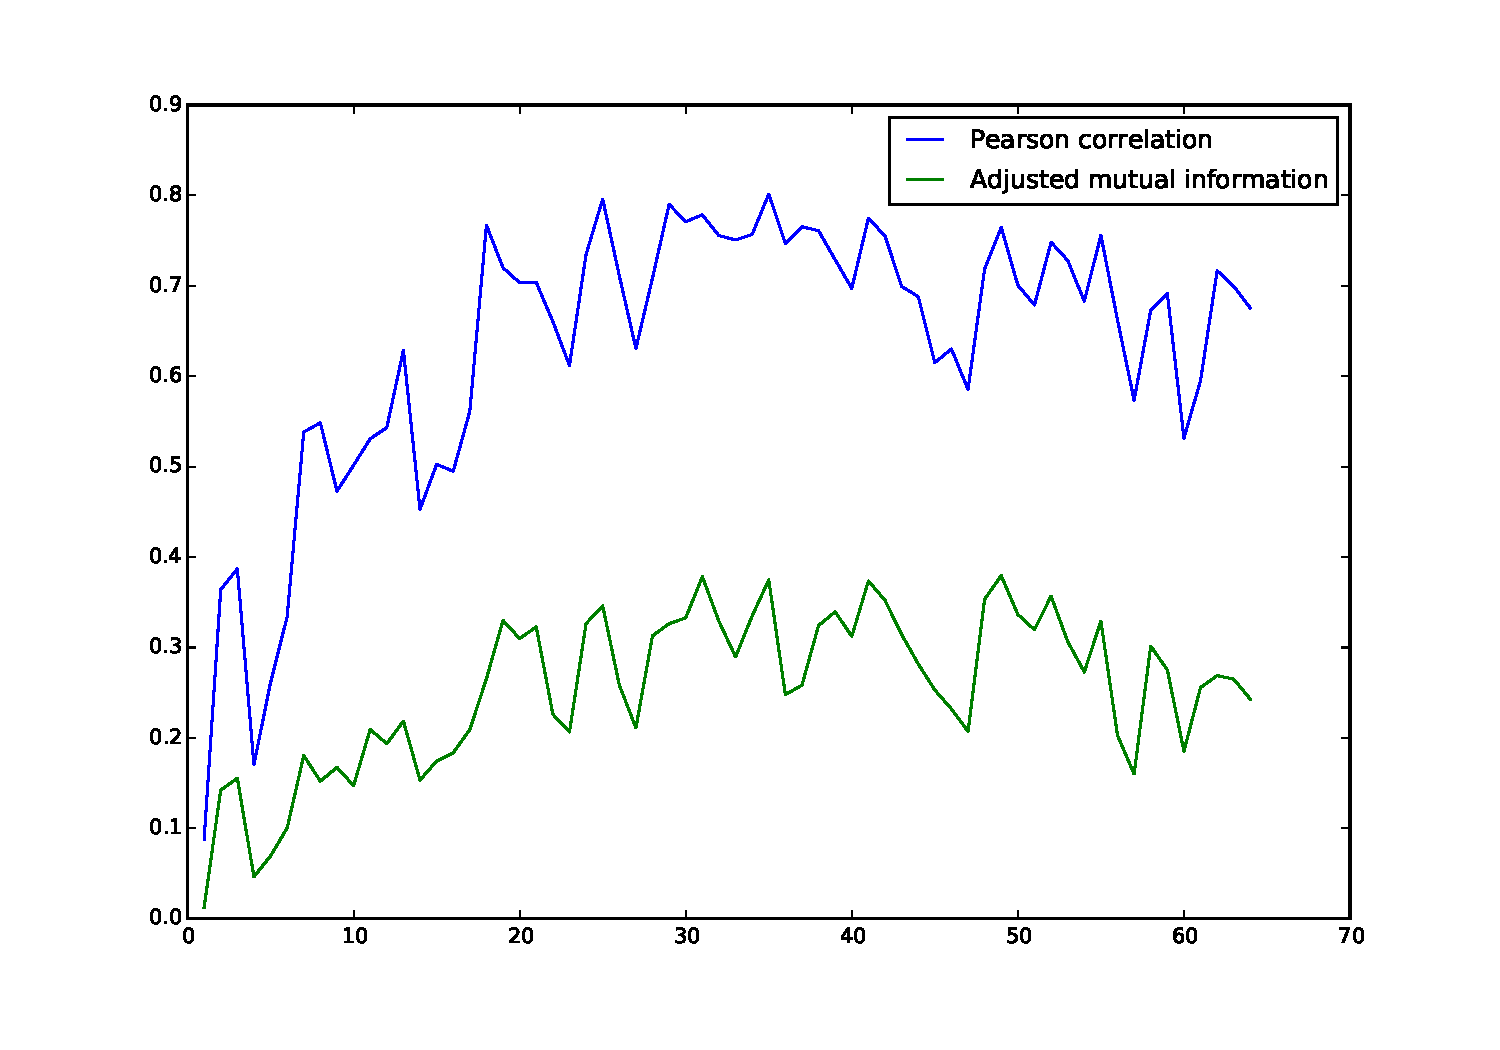
\includegraphics[width=.4\textwidth]{mi_pearson_watson.pdf}}
\caption{Adjusted mutual information and Pesrson correlation between word sets mostly related to John Watson during the time range.}\label{mi_pearson}
\end{figure}

\begin{figure}
\centerline{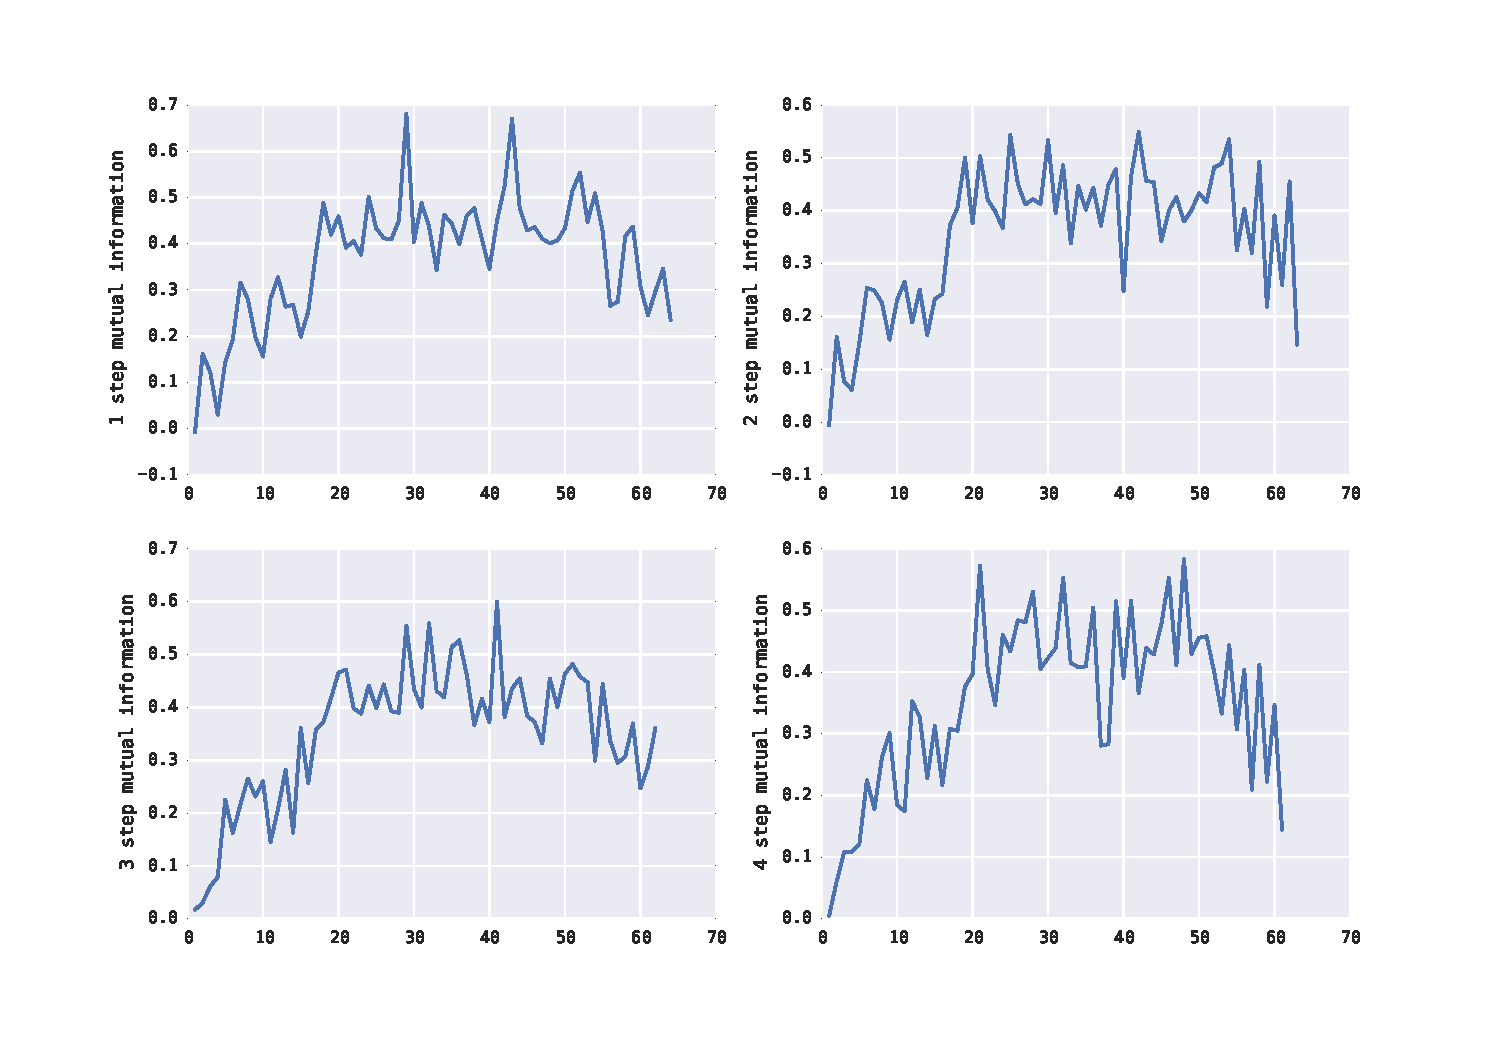
\includegraphics[width=.7\textwidth]{muti_step_mi_john.pdf}}
\caption{Adjusted mutual information between word sets mostly related to John Watson during the time range, with time step ranging from 1 to 4.}\label{multi_mi} 
\end{figure}


\subsection{Sentiment Analysis} Figure \ref{fleiss} shows the change of Fleiss' kappa between sentiment categorizations for writings concerning Sherlock Holmes during the time range. It can be found that after the early period, agreement level quickly rose and stabilized at a similar level, but decreased slightly at the latest period. However, it should also be noted that the agreement score remained slightly negative, which implies little agreement according to the conventional interpretation of this metric [cite Fleiss wiki again]. 


\begin{figure}
\centerline{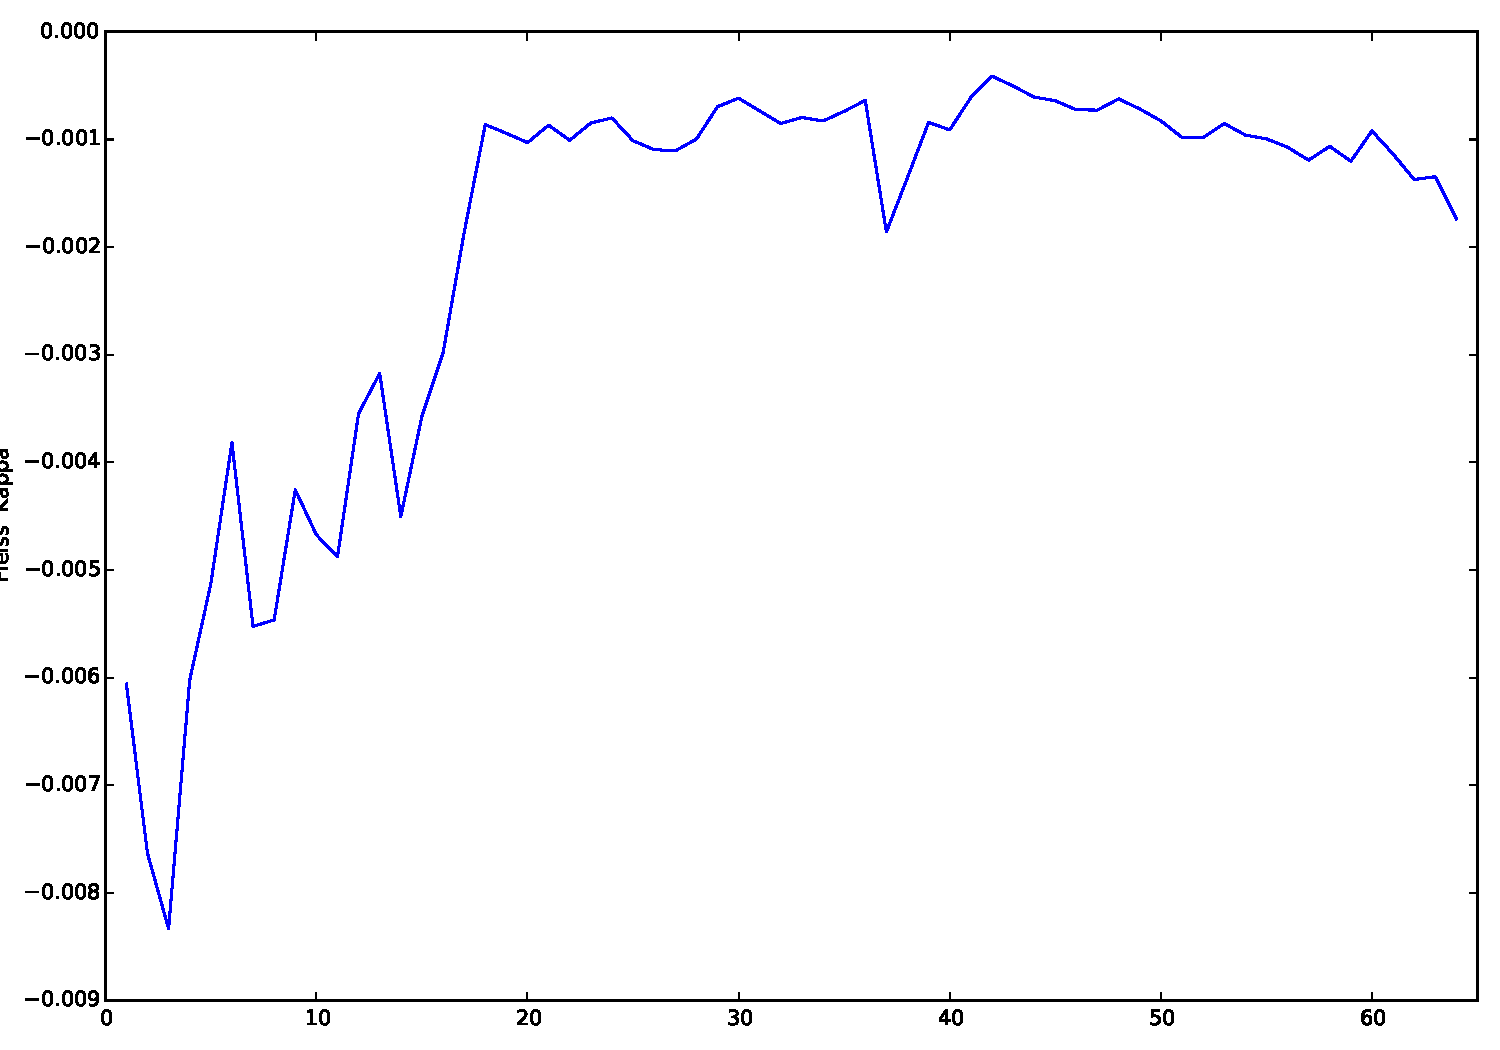
\includegraphics[width=.4\textwidth]{fleiss_kappa.pdf}}
\caption{Fleisss' Kappa of sentiment categories of writings about Sherlock Holmes during the time range..}\label{fleiss}
\end{figure}


\subsection{Tag Analysis} Here I plot the time distribution of the most popular tags, as identified by the method described above.  Figure \ref{freq_tag} shows the top words with highest frequency. It can be immediately noticed that these tags' distributions respond directly to the total count of works, which is plotted in Figure \ref{freq_tag_wtotal} for comparison. 
However, if we look at the tags that received most Kudos instead, the scenario becomes very different. The distribution of most of these tags shows clear peaks that are centered around certain time periods, and occurrence decrease significantly after those periods. 



\section{Discussion}
The analysis presented above suggests that this dataset has been able to cover the major life stages of the fandom, including origin, growth, peak and decline, according to the amount of transformative works procuced. In this case, transformative works begin to appear only a few days after the original work is published, and continue to grow in the next three years, with peaks happening every time a new season is broadcasted or DVDs are released. After the highest peak in early 2014, the amount of works begin to drop significantly. (It is likely that we will observe a revival when the 4th season is aired in 2016, but this falls outside the concern of this work). 

It seems possible that the agreement on characterization is, in some ways, related to the life period of the fandom. At least for the growing period, from Figure \ref{multi_mi} and Figure \ref{fleiss}, we are 


\section{Conclusion and Future Work}


\end{article}


\begin{figure}
\centerline{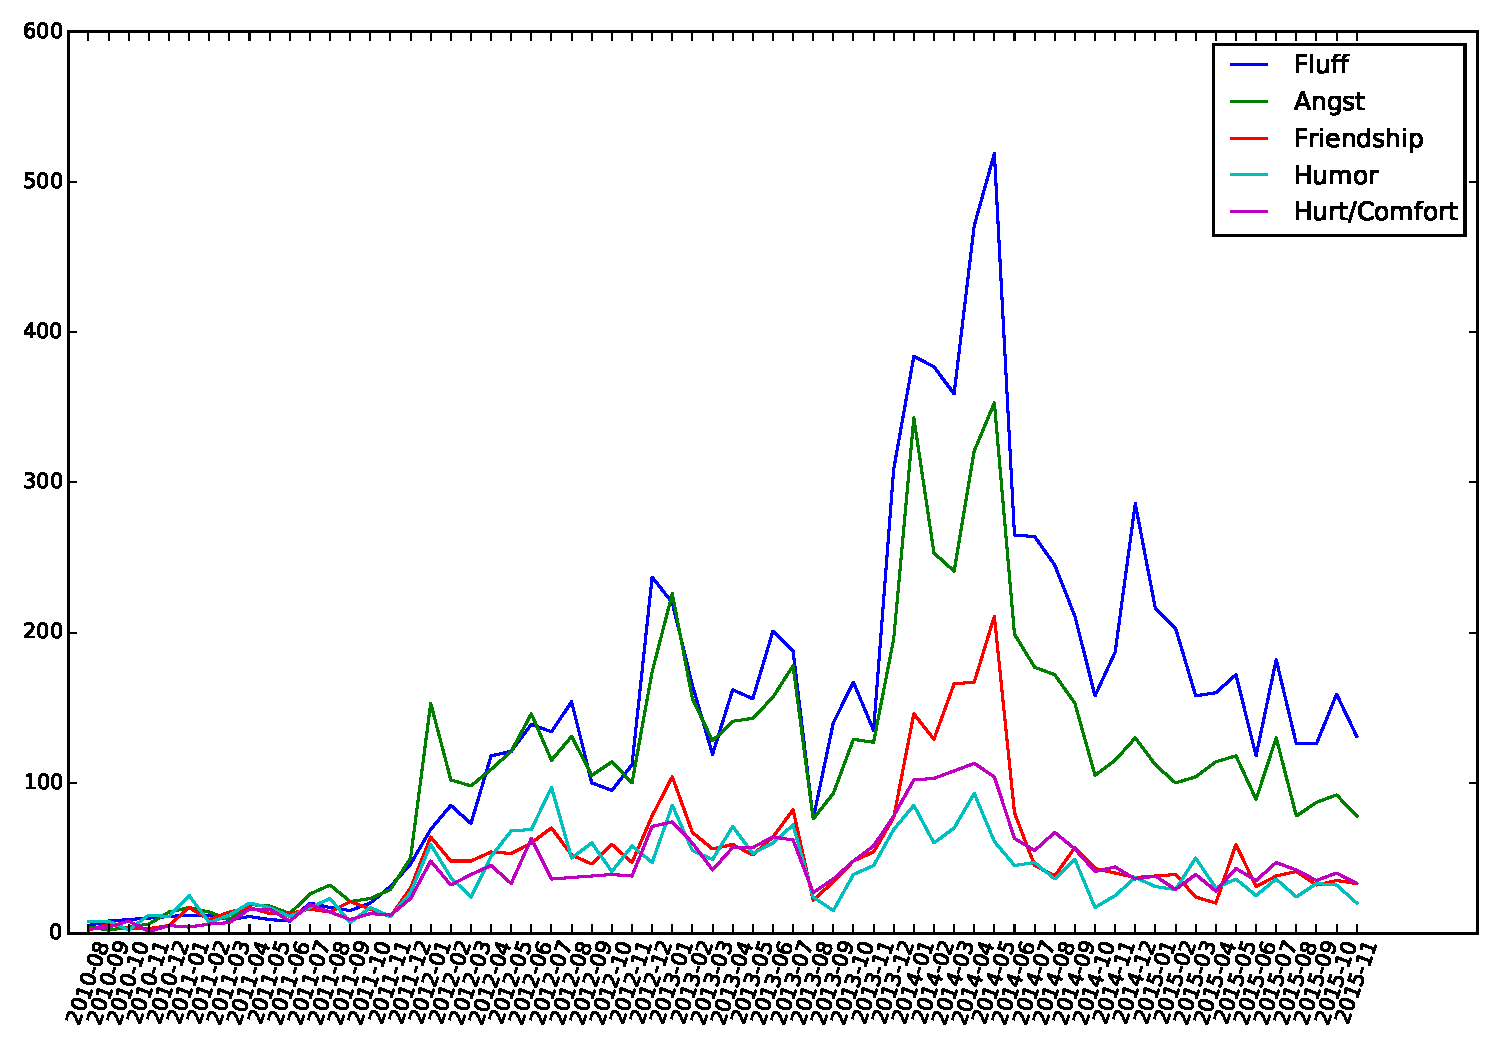
\includegraphics[width=.6\textwidth]{top_frequency_tag_time.pdf}}
\caption{Time distribution of top 5 tags according to total frequency of appearance.}\label{freq_tag}
\end{figure}

\begin{figure}
\centerline{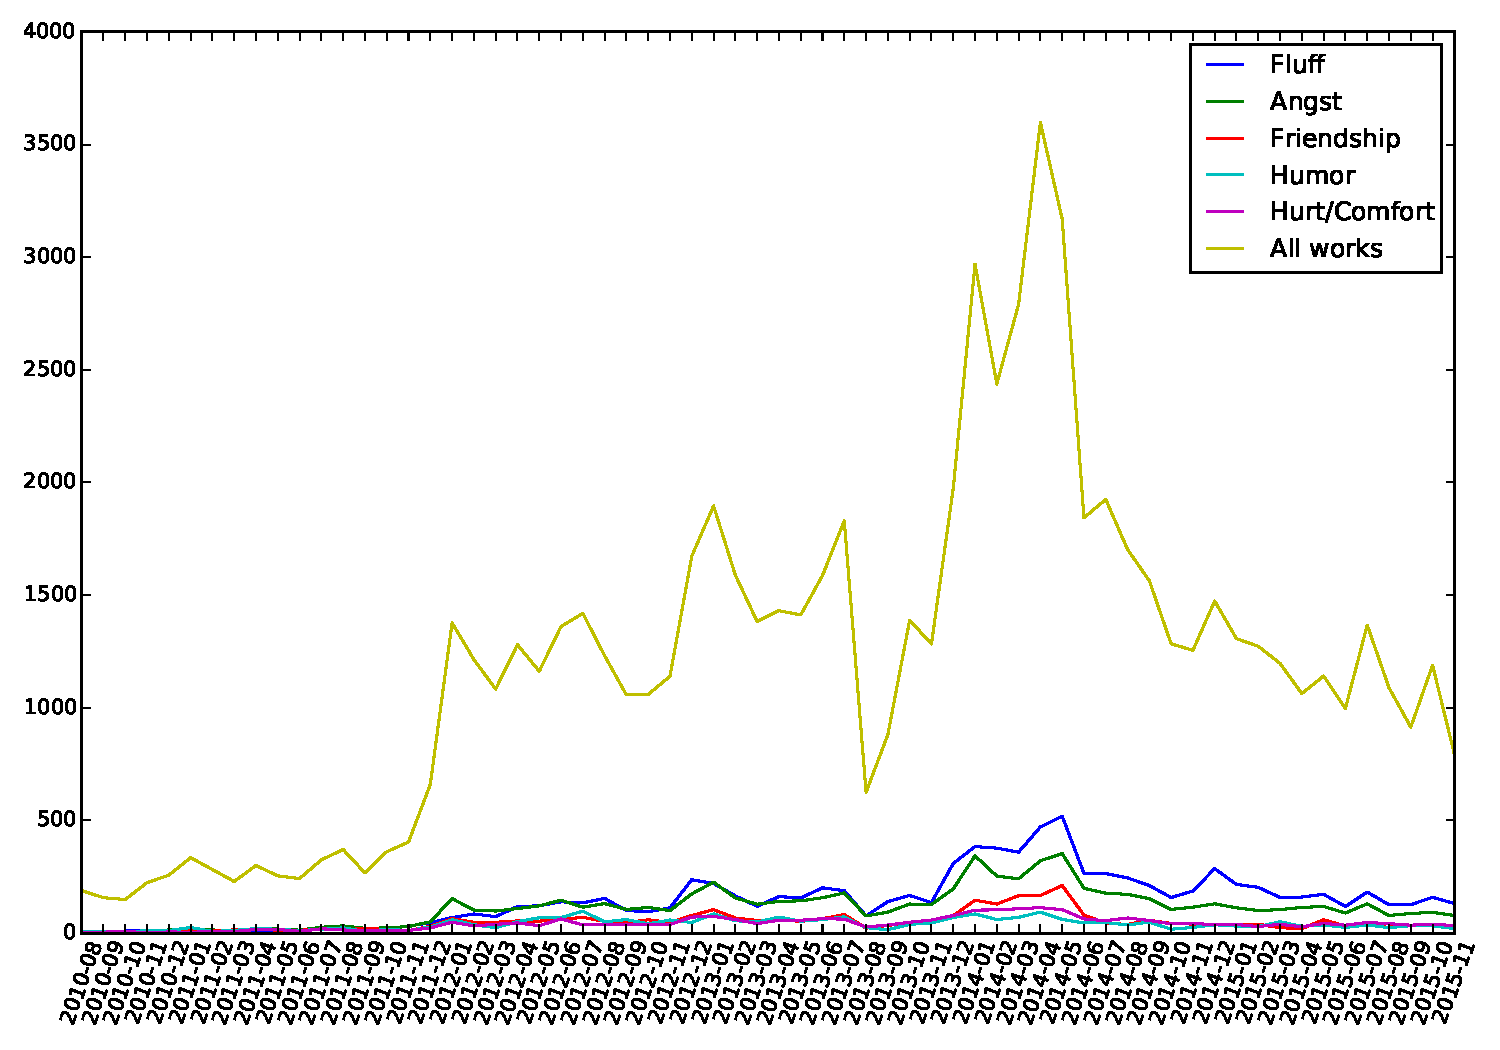
\includegraphics[width=.6\textwidth]{top_frequency_tag_time_w_total.pdf}}
\caption{Time distribution of top 5 tags identified by total frequency of appearance, as well as the number of works.}\label{freq_tag_wtotal}
\end{figure}

\begin{figure}
\centerline{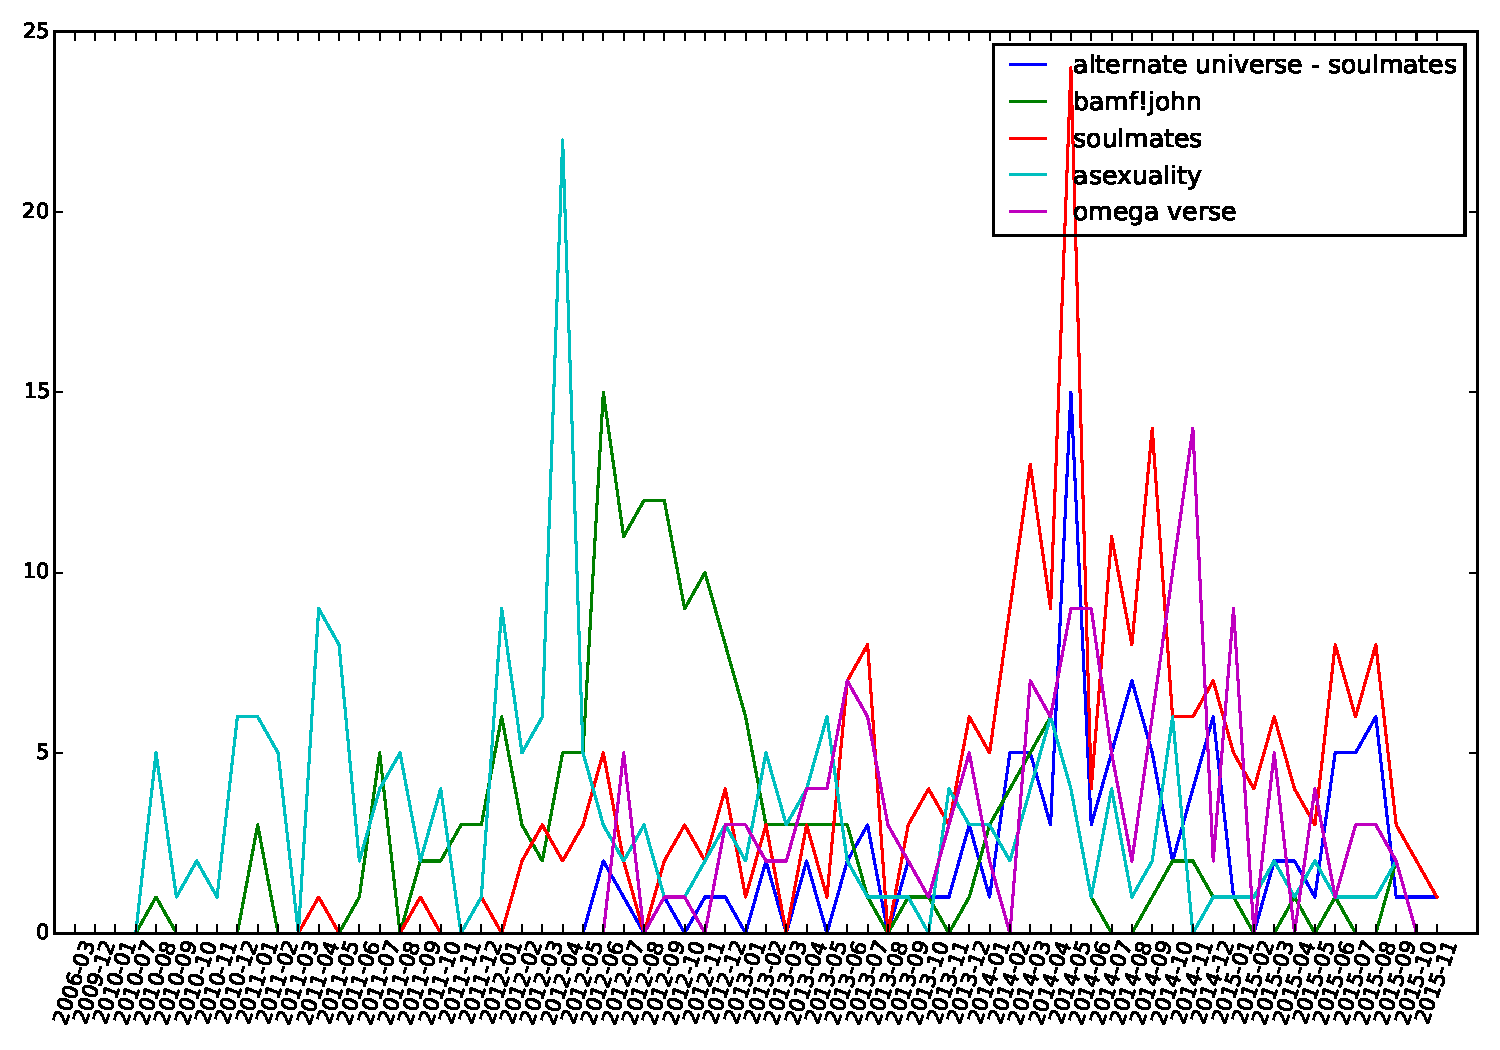
\includegraphics[width=.6\textwidth]{top_popularity_tag_time.pdf}}
\caption{Time distribution of top 5 tags identified by average Kudos.}\label{popular_tag}
\end{figure}

\begin{table}
\centering
\caption{Fields of AO3 work metadata}
\begin{tabular*}{\hsize}{@{\extracolsep{\fill}}lcr}
Metadata type&Fields\cr
\hline
Author generated&author, title, summary, fandom, \cr
 &characters, relationship, category, rating, \cr
 &additional tags, archive warnings, notes\cr
 \hline
System generated&publish date, complete date, chapter count,\cr
 & word count, bookmarks count, chapters count,\cr
  & hits, kudos, language, comment counts \cr
\hline
\end{tabular*}
\end{table}



\end{document}


